\documentclass[12pt,reqno]{amsart}
\usepackage[top=2cm, left=2cm,right=2cm,bottom=2cm]{geometry}
\renewcommand{\baselinestretch}{1.2}
\usepackage{amsmath}
\usepackage{amssymb}
\usepackage{scalefnt}
\usepackage{tikz}
\usepackage{color,hyperref,enumerate,multicol}
\definecolor{darkblue}{rgb}{0.0,0.0,0.3}
\hypersetup{colorlinks,breaklinks,
            linkcolor=darkblue,urlcolor=darkblue,
            anchorcolor=darkblue,citecolor=darkblue}
            
\usepackage{algorithm}
\usepackage{algorithmic}
\pagestyle{empty}
\newcommand{\N}{\ensuremath{\mathbb{N}}}
\newcommand{\Z}{\ensuremath{\mathbb{Z}}}
\newcommand{\R}{\ensuremath{\mathbb{R}}}
\newcommand{\bL}{\ensuremath{\mathbf{L}}}
\newcommand{\bP}{\ensuremath{\mathbf{P}}}
\newcommand{\bQ}{\ensuremath{\mathbf{Q}}}
\newcommand{\bA}{\ensuremath{\mathbf{A}}}
\newcommand{\bB}{\ensuremath{\mathbf{B}}}
\newcommand{\bG}{\ensuremath{\mathbf{G}}}
\newcommand{\bH}{\ensuremath{\mathbf{H}}}
\newcommand{\invG}{\ensuremath{\operatorname{inv}^{\bG}}}
\newcommand{\invH}{\ensuremath{\operatorname{inv}^{\bH}}}
\newcommand{\meet}{\ensuremath{\wedge}}
\newcommand{\Meet}{\ensuremath{\bigwedge}}
\newcommand{\<}{\ensuremath{\langle}}
\renewcommand{\>}{\ensuremath{\rangle}}
\newcommand{\join}{\ensuremath{\vee}}
\renewcommand{\emptyset}{\ensuremath{\varnothing}}
\renewcommand{\subset}{\ensuremath{\subsetneq}}
\newcommand{\boldemph}{\emph}
\newcommand{\lcm}{\operatorname{lcm}}

\newcommand{\probskip}{\vskip1cm}

\begin{document}
\thispagestyle{empty}

\noindent \textbf{Math 301} \hskip5cm {\bf Homework 9} \hfill {\bf Fall 2014}
\vskip1cm
\noindent {\bf Exercises:} 1, 2, 3 below and Judson: 9.22, 9.27, 9.31\\
{\bf Recommended:} 9.19, 9.21, 9.23, 9.41, 9.42, 9.45\\
{\bf Due date:} Friday, 10/31

\bigskip

\noindent The first few exercises require some definitions from lecture, 
repeated here for your convenience.

\vskip5mm

\noindent Let $\bA = \<A, F^{\bA}\>$ and $\bB = \<B, F^{\bB}\>$ be two algebras of the
same \emph{similarity type}.  That is, to each operation
symbol $f \in F$ there corresponds an operation $f^{\bA}$ defined on $\bA$ and an
operation $f^{\bB}$ defined on $\bB$.
Thus, the set of operations defined on $\bA$ is the set 
$F^{\bA} = \{f^{\bA} : f\in F\}$; similarly 
$F^{\bB} = \{f^{\bB} : f\in F\}$.

\vskip3mm

\noindent For example, any two groups $\bG$ and $\bH$ have the same similarity type. 
To emphasize this, we could denote the operations of these groups using
the precise (albeit somewhat awkward) notation of the previous paragraph, as follows:
\[
\bG  = \<G, \circ^{\bG}, \invG, e^{\bG}\> \quad \text{ and } \quad
\bH  = \<H, \circ^{\bH}, \invH, e^{\bH}\>.
\] 
Here $\circ^{\bG}$, $\invG$, and $e^{\bG}$ represent the \emph{interpretation
in} $\bG$ of the binary, unary (inverse), and  nullary (identity)
operations that a group must possess (similarly for $\bH$).  

\vskip5mm

\noindent An \emph{algebra homomorphism} (or simply \emph{homomorphism}), denoted by
$\varphi: \bA \rightarrow \bB$, is a function $\varphi$ with domain $A$ and
codomain $B$ that satisfies the following conditions: for each $f \in F$, if $f$
is an $n$-ary operation symbol, and if $a_1, \dots, a_n \in A$, then
\[
\varphi(f^{\bA}(a_1, \dots, a_n)) = f^{\bB}(\varphi(a_1), \dots, \varphi(a_n)).
\]

\vskip3mm

\noindent For example, a \emph{group homomorphism} $\varphi: \bG \rightarrow \bH$  is a function 
$\varphi$ with domain $G$ and codomain $H$ that satisfies, $\forall x, y \in G$,
\begin{enumerate}
\item  $\varphi(x\circ^{\bG} y) = \varphi(x) \circ^{\bH} \varphi(y)$,
\item  $\varphi(\invG(x)) = \invH(\varphi(x))$,
\item  $\varphi(e^{\bG}) = e^{\bH}$.
\end{enumerate}

\vskip5mm

\noindent The textbook defines a group \emph{isomorphism} to be a group homomorphism that is both
one-to-one and onto.  This definition is fine for algebraic structures (like
groups).  
It does not work, however, for relational structures, like posets. (See Exercise 3 below).
A definition that works for both algebraic and relational structures is the following:
A homomorphism $\varphi : \bA \rightarrow \bB$ is an \emph{isomorphism} if there
exists a homomorphism $\psi: \bB \rightarrow \bA$ that composes with
$\varphi$ to give the identity, that is,
$\varphi \circ \psi = \operatorname{id}_B$
and $\psi \circ \varphi= \operatorname{id}_A$. (Here, $\operatorname{id}_X$
denotes the identity function on the set $X$: $\operatorname{id}_X(x) = x$.)

\newpage

\noindent {\bf Exercises}

\begin{enumerate}[{\bf 1.}]
%% 1 %%%%%%%%%%%%%%%%%%%%%%%%%%%%%%%%%%%%%%%%%%%%%%%%
\item When discussing two groups, like $\bG$ and $\bH$ above,
  our textbook uses more convenient notation, such as 
  $(G, \cdot)$ and $(H, \circ)$ (or, even more simply, $G$ and $H$).  The book will then
  define a \emph{homomorphism} to be a function $\varphi: G\rightarrow H$ satisfying
  $\varphi(x\cdot y) = \varphi(x) \circ \varphi(y)$.
  Prove that this is equivalent to the definition given above by showing that 
  conditions (2) and (3) are unnecessary.\\
  \ [Hint: Assuming (1), derive (3), then derive (2).]

\vskip1cm

%% 2 %%%%%%%%%%%%%%%%%%%%%%%%%%%%%%%%%%%%%%%%%%%%%%%%
\item
Define a lattice homomorphism.
Then consider a lattice $\bL = \<L, \meet, \join\>$ and a poset $\bP = \<P, \preccurlyeq\>$.
Is it possible to define a homomorphism $\varphi: \bL \rightarrow \bP$?  Explain.

\vskip1cm

%% 3 %%%%%%%%%%%%%%%%%%%%%%%%%%%%%%%%%%%%%%%%%%%%%%%%
\item
A \emph{poset homomorphism} is an order preserving map.  That is, if
$\bP = \<P, \leqslant\>$ and 
$\bQ = \<Q, \preccurlyeq\>$ are two partially 
ordered sets, then a homomorphism 
$\varphi: \bP \rightarrow \bQ$  is a function satisfying, for all $x, y\in P$, 
if $x \leqslant y$ then $\varphi(x)\preccurlyeq \varphi(y)$.
Consider the two definitions of \emph{isomorphism} given in the last paragraph
on Page 1 above.
Using the two posets shown below, explain why the first of these definitions is 
not appropriate for posets.

\vskip5mm

\begin{center}
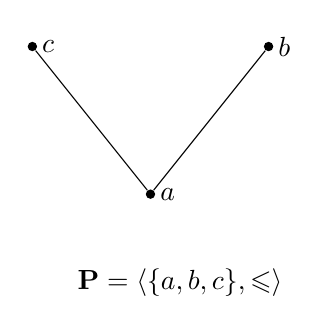
\begin{tikzpicture}[scale=0.75]
  \node (0) at (0,.5) [fill,circle,inner sep=1.2pt] {};
  \node (1) at (2,3) [fill,circle,inner sep=1.2pt] {};
  \node (2) at (-2,3) [fill,circle,inner sep=1.2pt] {};
  \draw (0) node [right] {$a$};
  \draw (1) node [right] {$b$};
  \draw (2) node [right] {$c$};
  \node (3) at (0.5,-1) {$\bP = \<\{a,b,c\},  \leqslant\>$};
  \draw (1) to (0) to (2);
\end{tikzpicture}
\hskip3cm
\begin{tikzpicture}[scale=0.75]
  \node (0) at (0,0) [fill,circle,inner sep=1.2pt] {};
  \node (1) at (0,2) [fill,circle,inner sep=1.2pt] {};
  \node (2) at (0,4) [fill,circle,inner sep=1.2pt] {};
  \draw (0) node [right] {$0$};
  \draw (1) node [right] {$1$};
  \draw (2) node [right] {$2$};
  \node (3) at (0.5,-1.5) {$\bQ = \<\{0,1,2\}, \preccurlyeq\>$};
  \draw (0) to (1) to (2);
\end{tikzpicture}
\end{center}

\vskip1cm

%% %% 7 %%%%%%%%%%%%%%%%%%%%%%%%%%%%%%%%%%%%%%%%%%%%%%%%
%% \item[{\bf 9.7.}] 
%% Show that any cyclic group of order $n$ is isomorphic to ${\mathbb Z}_n$. 

\vskip1cm

\item[{\bf 9.22}]
Let $G$ be a group of order 20. If $G$ has subgroups $H$ and $K$ of
orders 4 and 5 respectively such that $hk = kh$ for all $h \in H$ and
$k \in K$, prove that $G$ is the internal direct product of $H$ and $K$. 

\vskip1cm

\item[{\bf 9.27}]
Let $G \cong H$. Show that if $G$ is cyclic, then so is $H$.

\vskip1cm

\item[{\bf 9.31}]
Let $\phi : G_1 \rightarrow G_2$ and  $\psi : G_2 \rightarrow G_3$  be
isomorphisms. Show that  $\phi^{-1}$ and $\psi \circ \phi$ are both
isomorphisms. Using these results, show that the isomorphism of groups
determines an equivalence relation on the class of all groups.
 
\end{enumerate}
\end{document}




\item
Prove that ${\mathbb Z} \cong n{\mathbb Z}$ for $n \neq 0$.
 

\item
Prove that ${\mathbb C}^\ast$ is isomorphic to the subgroup of $GL_2(
{\mathbb R} )$ consisting of matrices of the form 
\[
\begin{pmatrix}
a & b \\
-b & a
\end{pmatrix}
\]
 

\item
Prove or disprove: $U(8) \cong {\mathbb Z}_4$.
 

\item
Prove that $U(8)$ is isomorphic to the group of matrices
\[
\begin{pmatrix}
1 & 0 \\
0 & 1
\end{pmatrix},
\begin{pmatrix}
1 & 0 \\
0 & -1
\end{pmatrix},
\begin{pmatrix}
-1 & 0 \\
0 & 1
\end{pmatrix},
\begin{pmatrix}
-1 & 0 \\
0 & -1
\end{pmatrix}.
\]
 

\item
Show that $U(5)$ is isomorphic to $U(10)$, but $U(12)$ is not.
 

\item
Show that the $n$th roots of unity are isomorphic to ${\mathbb Z}_n$. 
 

\item 
Show that any cyclic group of order $n$ is isomorphic to ${\mathbb Z}_n$. 
 

\item
Prove that ${\mathbb Q}$ is not isomorphic to ${\mathbb Z}$.
 

\item
Let $G = {\mathbb R} \setminus \{ -1 \}$ and define a binary operation on
$G$ by 
\[
a \ast b = a + b + ab.
\]
Prove that $G$ is a group under this operation. Show that $(G, *)$ is
isomorphic to the multiplicative group of nonzero real numbers.
 

\item
Show that the matrices
\begin{gather*}
\begin{pmatrix}
1 & 0 & 0 \\
0 & 1 & 0 \\
0 & 0 & 1
\end{pmatrix}
\quad
\begin{pmatrix}
1 & 0 & 0 \\
0 & 0 & 1 \\
0 & 1 & 0
\end{pmatrix}
\quad
\begin{pmatrix}
0 & 1 & 0 \\
1 & 0 & 0 \\
0 & 0 & 1
\end{pmatrix} \\
\begin{pmatrix}
0 & 0 & 1 \\
1 & 0 & 0 \\
0 & 1 & 0
\end{pmatrix}
\quad
\begin{pmatrix}
0 & 0 & 1 \\
0 & 1 & 0 \\
1 & 0 & 0
\end{pmatrix}
\quad
\begin{pmatrix}
0 & 1 & 0 \\
0 & 0 & 1 \\
1 & 0 & 0
\end{pmatrix}
\end{gather*}
form a group. Find an isomorphism of $G$ with a more familiar group of
order~6. 

 
\item
Find five non-isomorphic groups of order 8.
 

\item
Prove $S_4$ is not isomorphic to $D_{12}$.
 
% TWJ, 2010/04/21
% Made correction to exercise at the suggestion of C. Thon

\item
Let $\omega = \cis(2 \pi /n)$ be a primitive $n$th root of
unity.  Prove that the matrices 
\[
A=
\begin{pmatrix}
\omega & 0 \\
0 & \omega^{-1}
\end{pmatrix}
\quad \text{and} \quad
B =
\begin{pmatrix}
0 & 1 \\
1 & 0
\end{pmatrix}
\]
generate a multiplicative group isomorphic to $D_n$.
 

\item
Show that the set of all matrices of the form
\[
\begin{pmatrix}
\pm 1 & k\\
0 & 1
\end{pmatrix},
\]
is a group isomorphic to $D_n$, where all entries in the matrix are in ${\mathbb Z}_n$.

%TWJ 10/21/2012
%Statement of exercise corrected.  Suggested by R. Beezer and B. Whetter.
 

\item
List all of the elements of ${\mathbb Z}_4 \times {\mathbb Z}_2$.
 

\item
Find the order of each of the following elements.

\begin{enumerate}
 
 \item
$(3, 4)$ in ${\mathbb Z}_4 \times {\mathbb Z}_6$

 \item
$(6, 15, 4)$ in ${\mathbb Z}_{30} \times {\mathbb Z}_{45} \times {\mathbb
Z}_{24}$

 \item
$(5, 10, 15)$ in ${\mathbb Z}_{25} \times {\mathbb Z}_{25} \times {\mathbb
Z}_{25}$

 \item
$(8, 8, 8)$ in ${\mathbb Z}_{10} \times {\mathbb Z}_{24} \times {\mathbb
Z}_{80}$
 
\end{enumerate}
 

\item
Prove that $D_4$ cannot be the internal direct product of two of its
proper subgroups. 
 

\item
Prove that the subgroup of ${\mathbb Q}^\ast$ consisting of elements of
the form $2^m 3^n$ for $m,n \in {\mathbb Z}$ is an internal direct
product isomorphic to ${\mathbb Z} \times {\mathbb Z}$.
 

\item
Prove that $S_3 \times {\mathbb Z}_2$ is isomorphic to $D_6$. Can you
make a conjecture about $D_{2n}$? Prove your conjecture. [\emph{Hint:}
Draw the picture.] 
 

\item
Prove or disprove: Every abelian group of order divisible by 3
contains a subgroup of order 3.  


\item
Prove or disprove: Every nonabelian group of order divisible by 6
contains a subgroup of order 6. 
 

\item
Let $G$ be a group of order 20. If $G$ has subgroups $H$ and $K$ of
orders 4 and 5 respectively such that $hk = kh$ for all $h \in H$ and
$k \in K$, prove that $G$ is the internal direct product of $H$ and $K$. 
 

\item
Prove or disprove the following assertion. Let $G$, $H$, and $K$ be
groups. If $G \times K \cong H \times K$, then $G \cong H$. 
 

\item
Prove or disprove: There is a noncyclic abelian group of order 51. 
 

\item
Prove or disprove: There is a noncyclic abelian group of order 52. 
 
%*****************************Theory
 

\item
Let $\phi : G_1 \rightarrow G_2$ be a group isomorphism. Show that
$\phi( x) = e$ if and only if $x=e$. 
 

\item
Let $G \cong H$. Show that if $G$ is cyclic, then so is $H$.
 

\item
Prove that any group $G$ of order $p$, $p$  prime, must be isomorphic
to ${\mathbb Z}_p$. 
 

\item
Show that $S_n$ is isomorphic to a subgroup of $A_{n+2}$.  

\item
Prove that $D_n$ is isomorphic to a subgroup of $S_n$.
 

\item
Let $\phi : G_1 \rightarrow G_2$ and  $\psi : G_2 \rightarrow G_3$  be
isomorphisms. Show that  $\phi^{-1}$ and $\psi \circ \phi$ are both
isomorphisms. Using these results, show that the isomorphism of groups
determines an equivalence relation on the class of all groups.
 

\item
Prove $U(5) \cong {\mathbb Z}_4$. Can you generalize this result to show
that $U(p) \cong {\mathbb Z}_{p-1}$? 
 

\item
Write out the permutations associated with each element of $S_3$ in
the proof of Cayley's Theorem. 
 
%*****************Automorphisms
 

\item
An \boldemph{automorphism}\index{Automorphism!of a
group}\index{Group!automorphism of} of a group $G$ is an isomorphism
with itself. Prove that complex conjugation is an automorphism of the
additive group of complex numbers; that is, show that the map $\phi(
a + bi ) = a - bi$ is an isomorphism from ${\mathbb C}$ to ${\mathbb C}$. 
 

\item
Prove that $a + ib \mapsto a - ib$ is an automorphism of ${\mathbb C}^*$. 
 

\item
Prove that $A \mapsto B^{-1}AB$ is an automorphism of $SL_2({\mathbb R})$
for all $B$ in $GL_2({\mathbb R})$. 
 

\item
We will denote the set of all automorphisms of $G$ by
$\aut(G)$\label{noteauto}.  Prove that  $\aut(G)$ is a subgroup of
$S_G$, the group of permutations of $G$. 
 

\item
Find $\aut( {\mathbb Z}_6)$.
 

\item
Find $\aut( {\mathbb Z})$.
 

\item
Find two nonisomorphic groups $G$ and $H$ such that 
$\aut(G) \cong \aut(H)$. 
 

\item
Let $G$ be a group and $g \in G$. Define a map $i_g : G \rightarrow
G$\label{noteinner} 
by $i_g(x) = g x g^{-1}$.  Prove that $i_g$ defines an automorphism of
$G$.  Such an automorphism is called an \boldemph{inner
automorphism}\index{Automorphism!inner}. The set of all inner
automorphisms is denoted by $\inn(G)$\label{noteinneraut}. 
 

\item
Prove that $\inn(G)$ is a subgroup of $\aut(G)$.
 

\item
What are the inner automorphisms of the quaternion group $Q_8$? Is
$\inn(G) = \aut(G)$ in this case? 
 

\item
Let $G$ be a group and $g \in G$.  Define maps $\lambda_g :G
\rightarrow G$ and $\rho_g :G \rightarrow G$\label{noterightreg}
 by $\lambda_g(x) = gx$
and $\rho_g(x) = xg^{-1}$. Show that $i_g = \rho_g \circ \lambda_g$ is
an automorphism of $G$. The isomorphism $g \mapsto \rho_g$ is called
the \boldemph{right regular representation}\index{Right regular
representation} of $G$. 
% Fixed the definition of right regular representation.  Suggested by Z. Teitler.
% TWJ - 12/19/2011
 

\item
Let $G$ be the internal direct product of subgroups $H$ and $K$.  Show
that the map $\phi : G \rightarrow H \times K$ defined by  $\phi(g) =
(h,k)$ for $g =hk$,  where $h \in H$ and  $k \in K$, is one-to-one and
onto. 
 

\item
Let $G$ and $H$ be isomorphic groups. If $G$ has a subgroup of order
$n$, prove that $H$ must also have a subgroup of  order $n$.
 

\item
If $G \cong \overline{G}$ and $H \cong \overline{H}$, show that $G
\times H \cong \overline{G} \times \overline{H}$.
 

\item
Prove that $G \times H$ is isomorphic to $H \times G$.
 

\item
Let $n_1, \ldots, n_k$ be positive integers. Show that
\[
\prod_{i=1}^k {\mathbb Z}_{n_i} \cong {\mathbb Z}_{n_1 \cdots n_k}
\]
if and only if $\gcd( n_i, n_j) =1$ for $i \neq j$.
 

\item
Prove that $A \times B$ is abelian if and only if $A$ and $B$ are
abelian. 
 

\item
If $G$ is the internal direct product of $H_1, H_2, \ldots, H_n$,
prove that $G$ is isomorphic to $\prod_i H_i$. 
 

\item
Let $H_1$ and $H_2$ be subgroups of $G_1$ and $G_2$, respectively. Prove that $H_1 \times H_2$ is a subgroup of $G_1 \times G_2$. 
 

\item % Change from \cong to equality suggested by Z. Teitler - TWJ 12/19/2011
Let $m, n \in {\mathbb Z}$. Prove that $\langle m,n \rangle = \langle d \rangle$ if and only if $d = \gcd(m,n)$.
 

\item  %Correction suggested by K. Brooks. - TWJ 11/21/2011
% Change from \cong to equality suggested by Z. Teitler - TWJ 12/19/2011
Let $m, n \in {\mathbb Z}$. Prove that $\langle m \rangle \cap \langle n \rangle = \langle l \rangle$ if and only if $l = \lcm(m,n)$. 

\item %Exercise suggested by R. Beezer. - TWJ 8/30/2011
\textbf{Groups of order $2p$.}
In this series of exercises we will classify all groups of order $2p$, where $p$ is an odd prime.
\begin{enumerate}

\item
Assume $G$ is a group of order $2p$, where $p$ is an odd prime.  If $a \in G$, show that $A$ must have order 1, 2, $p$, or $2p$.


\item
Suppose that $G$ an element of order $2p$.  Prove that $G$ isomorphic to ${\mathbb Z}_{2p}$.  Hence, $G$ is cyclic.



\item
Suppose that $G$ does not contain an element of order $2p$.  Show that $G$ must contain an element of order $p$.  \emph{Hint}:  Assume that $G$ does not contain an element of order $p$.



\item
Suppose that $G$ does not contain an element of order $2p$.  Show that $G$ must contain an element of order 2. 



\item
Let $P$ be a subgroup of $G$ with order $p$ and $y \in G$ have order 2.  Show that $yP = Py$.



\item
Suppose that $G$ does not contain an element of order $2p$ and $P = \langle z \rangle$ is a subgroup of order $p$ generated by $z$.  If $y$ is an element of order 2, then $yz = z^ky$ for some $2 \leq k < p$.



\item
Suppose that $G$ does not contain an element of order $2p$.  Prove that $G$ is not abelian.



\item
Suppose that $G$ does not contain an element of order $2p$ and $P = \langle z \rangle$ is a subgroup of order $p$ generated by $z$ and $y$ is an element of order 2.
Show that we can list the elements of $G$ as $\{z^iy^j\mid 0\leq i < p, 0\leq j < 2\}$.



\item
Suppose that $G$ does not contain an element of order $2p$ and $P = \langle z \rangle$ is a subgroup of order $p$ generated by $z$ and $y$ is an element of order 2.  Prove that the product
$(z^iy^j)(z^ry^s)$ can be expressed as a uniquely as $z^m y^n$ for some non negative integers $m, n$.  Thus, conclude that there is only one possibility for a non-abelian group of order $2p$, it must therefore be the one we have seen already, the dihedral group.



 
\end{enumerate}
